\chapter{Main memory}

This section provide a smart way to use all the powerful of the hardware you bought, the main focus is on the \textbf{main memory}. 

We saw at the begin of the course that a program, stored into the disk, became a process when it be brought from disk into main memory. 

Main memory and registers are the only storage that the CPU can access directly. Memory unit only sees a stream of:

\begin{itemize}
    \item addresses + read requests, or
    \item address + data and write requests
\end{itemize}

The CPU can access to the registers in one, or less, CPU clock. However, when the CPU takes data from the main memory it use many clock cycles, causing \textbf{stall}.

Cache sits between the main memory and the registers to provide a buffer of the needed data, we don't want a bottleneck.

\begin{figure}[htbp]
    \centering
    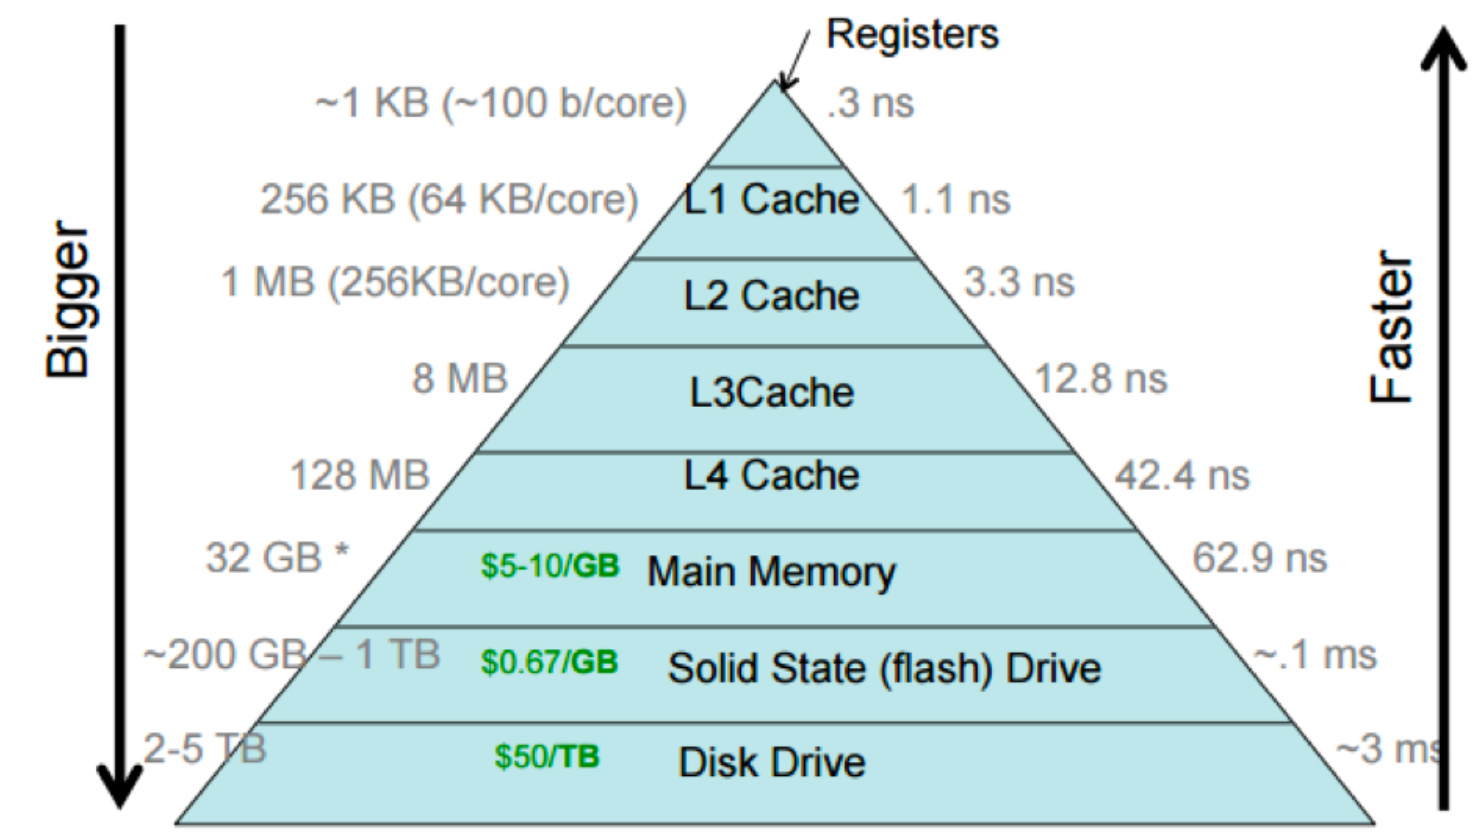
\includegraphics[width=0.6\linewidth]{img/memory.png}
    \caption{The Memories at a Glance, price and latency is higher than 2024 }
\end{figure}

All this levels contains a copy of the same subset of data.

\newpage
\subsection{Spatial Locality and Temporal Locality}

\paragraph{Spatial Locality:} Spatial Locality means that if I read a variable or instruction in memory, all the nearby data have a high chances to be fetched, so when I reed, I reed in blocks and store all the data into a faster memory.

\paragraph{Temporal Locality:} Temporal Locality means that if I read a variable the probability of reuse it is high, so I keep it in the cache memory.


\begin{figure}[htbp]
    \centering
    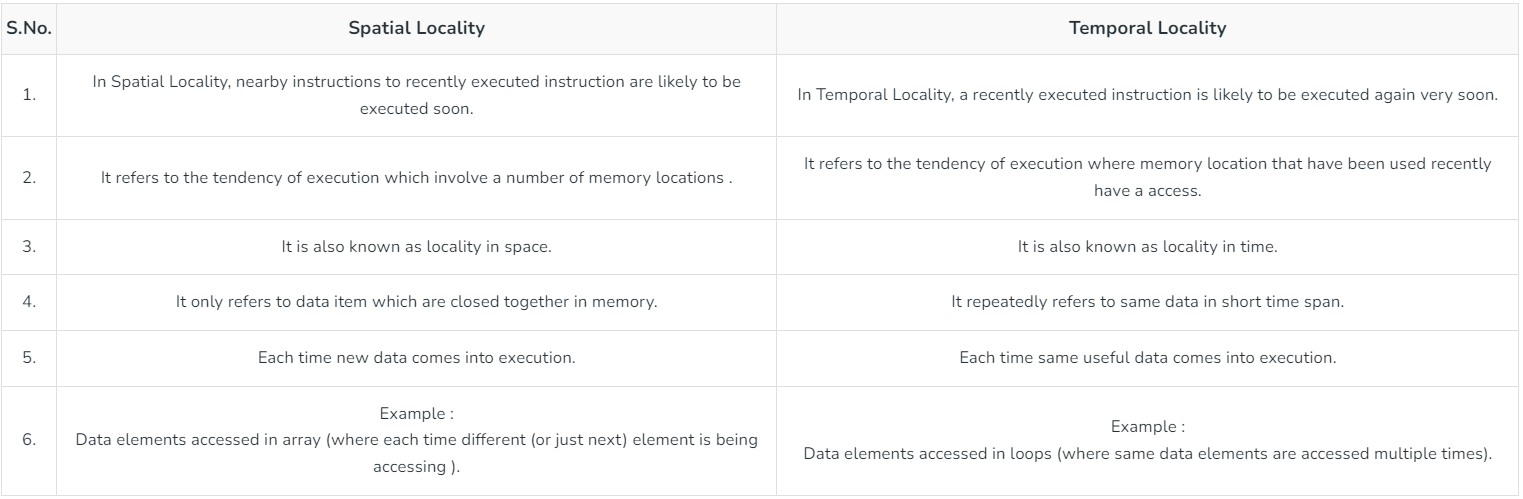
\includegraphics[width=1\linewidth]{img/spatial.png}
\end{figure}


\section{Protection}

When a program has became a process, all or most of its data are store in main memory. We need a way to:

\begin{itemize}
    \item Split the memory to all the process;
    \item Need to ensure that a process can access only the addresses in its address space.
\end{itemize}

We can provide to solve these problems by using a pair of \textbf{base} and \textbf{limit} registers define the logical address space of a process.


\begin{figure}[htbp]
    \centering
    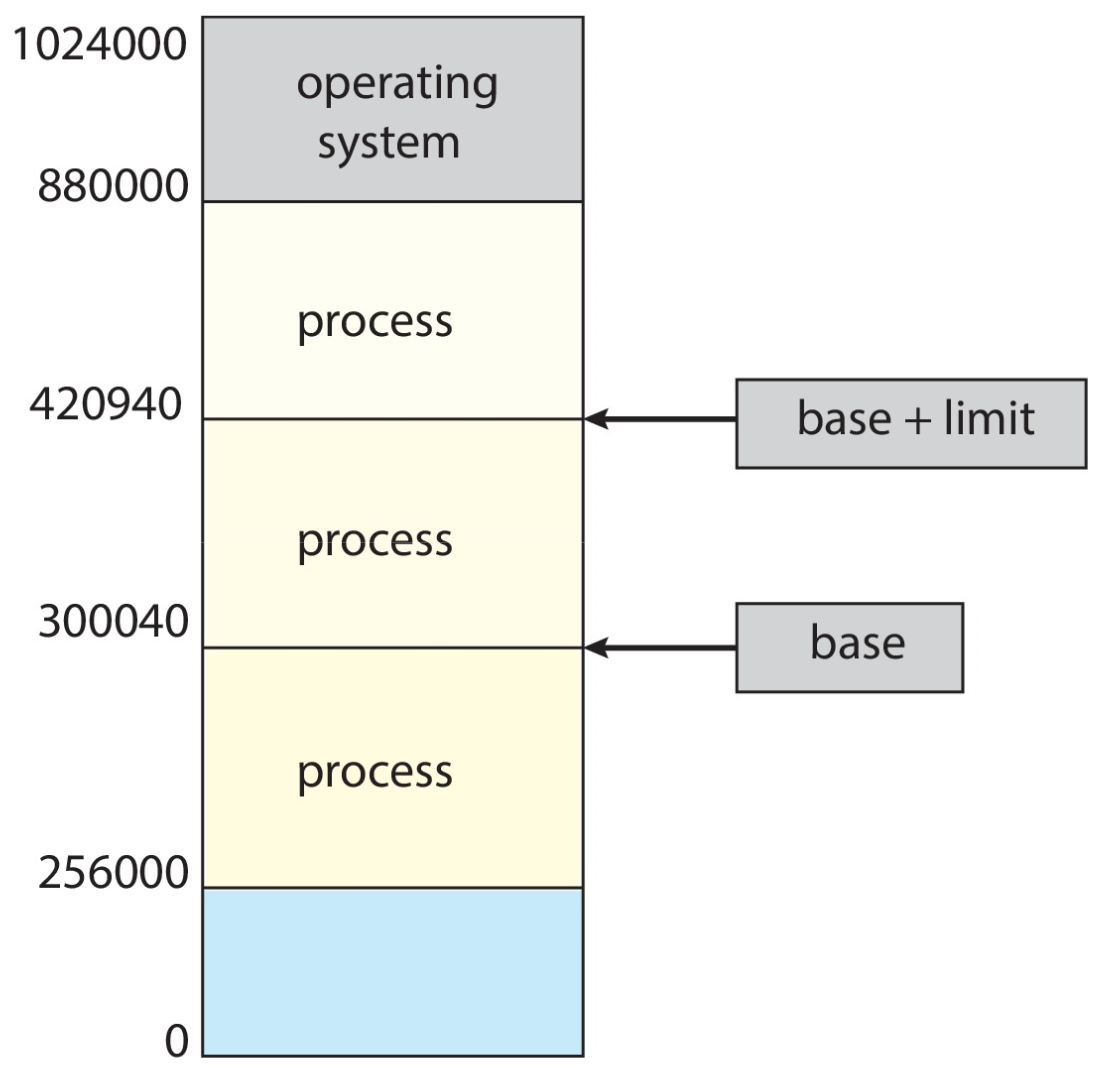
\includegraphics[width=0.4\linewidth]{img/adsfcv.png}
\end{figure}

\newpage
\subsection{Hardware Address Protection}
CPU/OS must check every memory access generated in user mode to
be sure it is between base and limit for that user.

\begin{figure}[htbp]
    \centering
    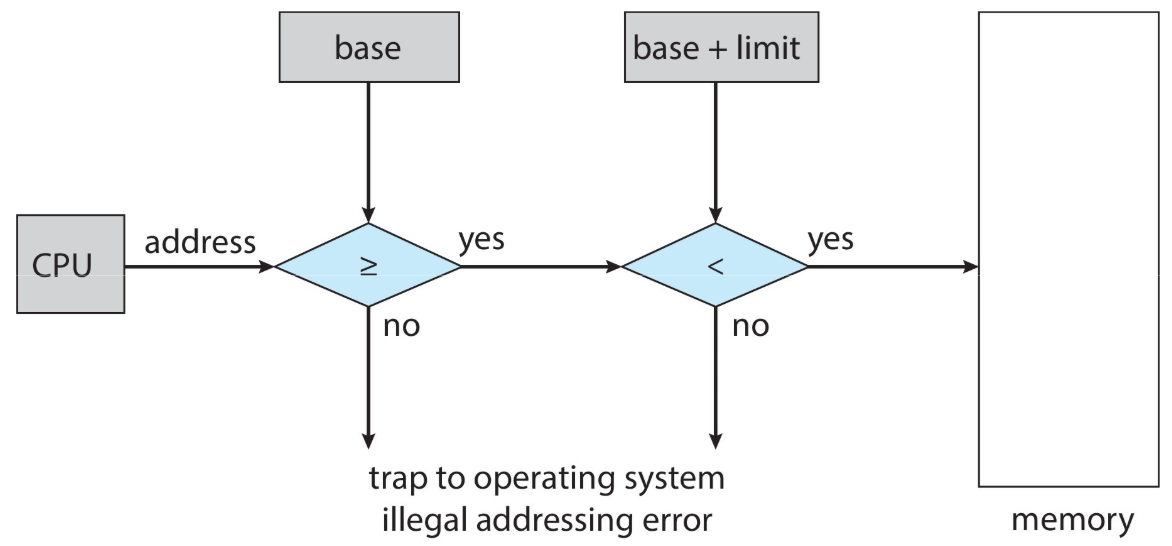
\includegraphics[width=0.6\linewidth]{img/ikadsuhc.png}
\end{figure}

The instructions to loading the base and limit registers are privileged.

\subsection{Address Binding}
When we crate a C program we do not take care about where the variable is in memory, we know only that it is in memory.

\begin{itemize}
    \item Source code addresses usually symbolic;
    \item Compiled code addresses bind to relocatable addresses, '14 bytes from beginning of this module', Instead of “byte 14';
    \item Linker or loader will bind relocatable addresses to absolute addresses;
    \item Each binding maps one address space to another.
\end{itemize}

In the compile code we see how many space we need and not the hard coded address. We want a dynamically bind and not static.

\newpage
\subsubsection{Binding of Instructions and Data to Memory}

When a program is started, the OS give an amount of space for the program. 

Address binding of instructions and data to memory addresses can happen at three different stages:

\begin{itemize}
    \item \textbf{Compile time:} If memory location known a priori, absolute code can be generated; must recompile code if starting location changes, used in embedded systems, or systems where the tasks are known a priori and are of a small number;

    \item \textbf{Load time:} Must generate relocatable code if memory location
is not known at compile time; Widely used strategy for old OSs or simple systems like dishwasher...


    \item Execution time: Binding delayed at run time if the process can
be moved while executing from one memory segment to another; Need hardware support (e.g., base and limit registers) and this is the De-facto standard for modern OSs.

\end{itemize}


\begin{figure}[htbp]
    \centering
    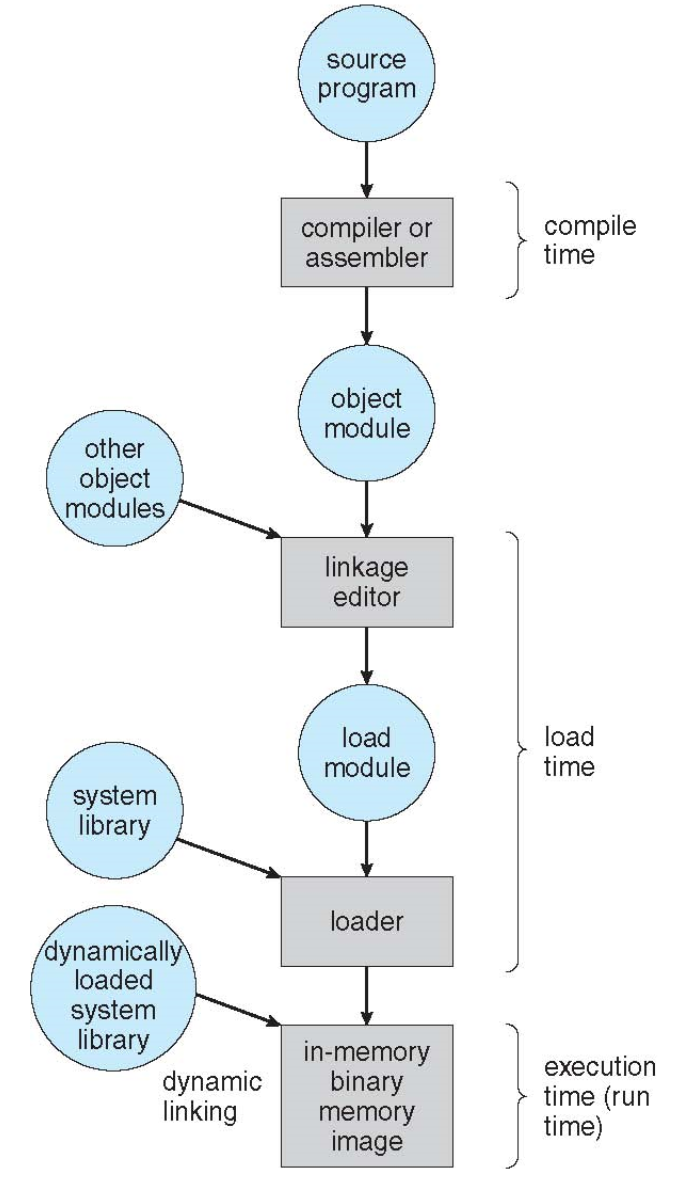
\includegraphics[width=0.4\linewidth]{img/rwefbg.png}
    \caption{Multistep Processing of a User Program }
\end{figure}


\newpage
\section{MEMORY MANAGEMENT UNIT - MMU}

I need a method to pass from virtual memory to hardware memory and vice versa, the \textbf{binding process}.

\subsection{Logical vs. Physical Address Space}
The concept of a logical address space that is bound to a separate \textbf{physical address space} is central to proper memory management.

\begin{itemize}
    \item \textbf{Logical address} – generated by the CPU; also referred to as \textbf{virtual address};
    \item \textbf{Physical address} – address seen by the memory unit.
\end{itemize}

Logical and physical addresses are the same in compile-time and
load-time address-binding schemes, but Logical (virtual) and physical addresses differ in execution-time
address-binding scheme.


\subsection{MMU}
Hardware device that at run time maps virtual to physical address

\begin{figure}[htbp]
    \centering
    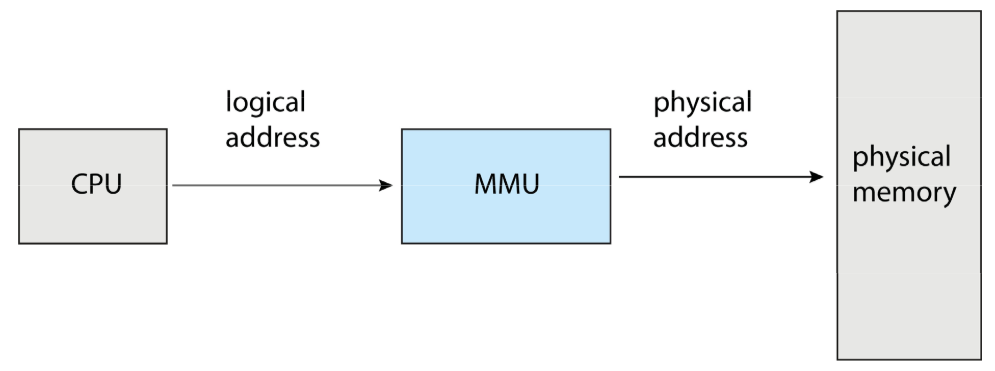
\includegraphics[width=0.65\linewidth]{img/hnter.png}
\end{figure}

The base register now called relocation register. The value in the relocation register is added to every address
generated by a user process at the time it is sent to memory.

\begin{figure}[htbp]
    \centering
    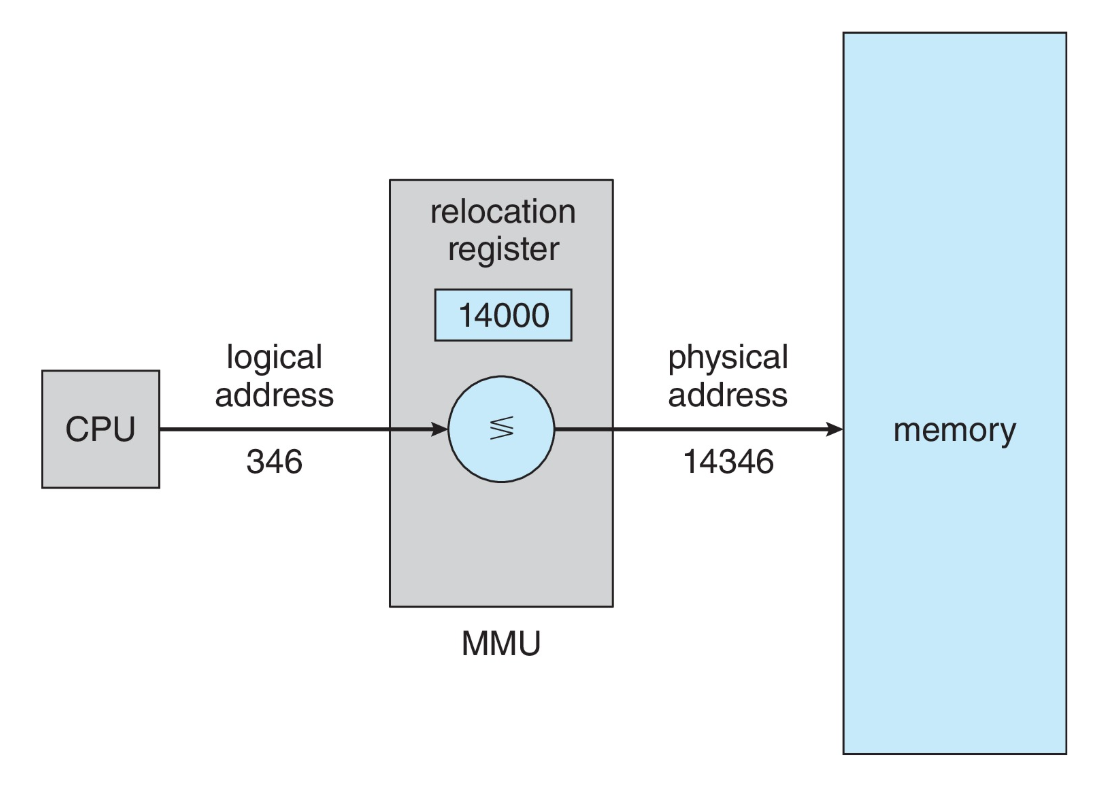
\includegraphics[width=0.6\linewidth]{img/mmuu.png}
\end{figure}

The user program deals with logical addresses; it \textbf{never sees the real physical addresses}. If you print the address of a variable in C program, it print the logical value and not the hardware real value!

\newpage
\subsection{Big programs + No Memory Space}
What if I have to execute a program that needs 1GB of memory, and I have only 200MB available?

The easiest solution is: throw an error like "No more main memory". But this is not a solution!

\section{LINKING AND LOADING}

\subsection{Dynamic loading}
The entire program does need to be in memory to execute. Routine (part of program) is not loaded until it is called this improve memory-space utilization; unused routine is never loaded. OS can help by providing libraries to implement dynamic loading.

\subsection{Static vs Dynamic Linking}
\textbf{Static linking} – system libraries and program code combined by the loader into the binary program image at compile-time.


\textbf{Dynamic linking} – linking postponed until execution time.
\paragraph{}
Small piece of code, stub, used to locate the appropriate memoryresident library routine. Stub replaces itself with the address of the routine, and executes the
routine at runtime, Operating system checks if the routine is in processes’ memory address, if not in address space, add to address space.

\paragraph{}
Dynamic linking is particularly useful for libraries, System also seen as “shared libraries”, this provide small programme because the library are shared by other programme.

\begin{figure}[htbp]
    \centering
    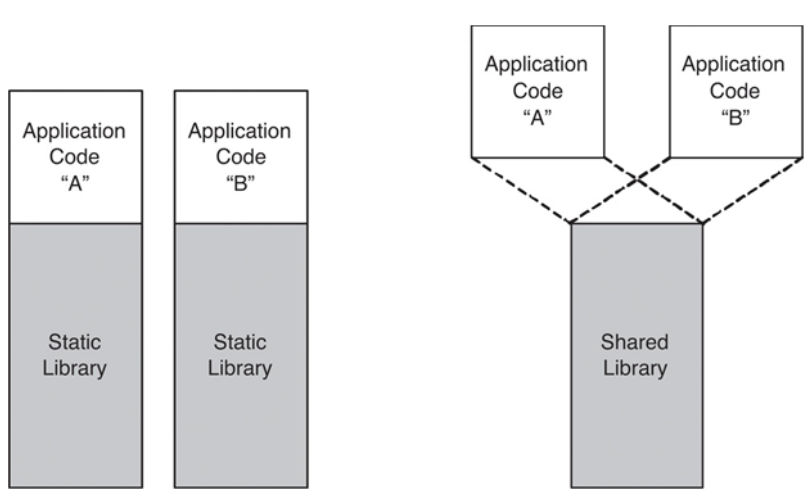
\includegraphics[width=0.55\linewidth]{img/ddl.png}
    \caption{.ddl file}
\end{figure}

Also this method provide an advantage: when the Windows update one library we must compile only this code and not all the other applications that use it.

\newpage
\section{Program allocation}

\subsection{Contiguous Allocation}

We want to manage efficiently the main memory because main memory must support both OS and user processes and limited resource, must allocate efficiently. 

Contiguous allocation is one early method, arrays and linked lists.

\paragraph{}

Main memory usually into two partitions:

\begin{itemize}
    \item Resident operating system, usually held in low memory with interrupt vector;
    \item User processes then held in high memory
\end{itemize}

Each process contained in single contiguous section of memory. 

Relocation registers used to protect user processes from each other, and from changing operating-system code and data

\begin{itemize}
    \item Base register contains value of smallest physical address
    \item Limit register contains range of logical addresses – each logical address must be less than the limit register
    \item MMU maps logical address dynamically
\end{itemize}


 \begin{figure}[htbp]
     \centering
     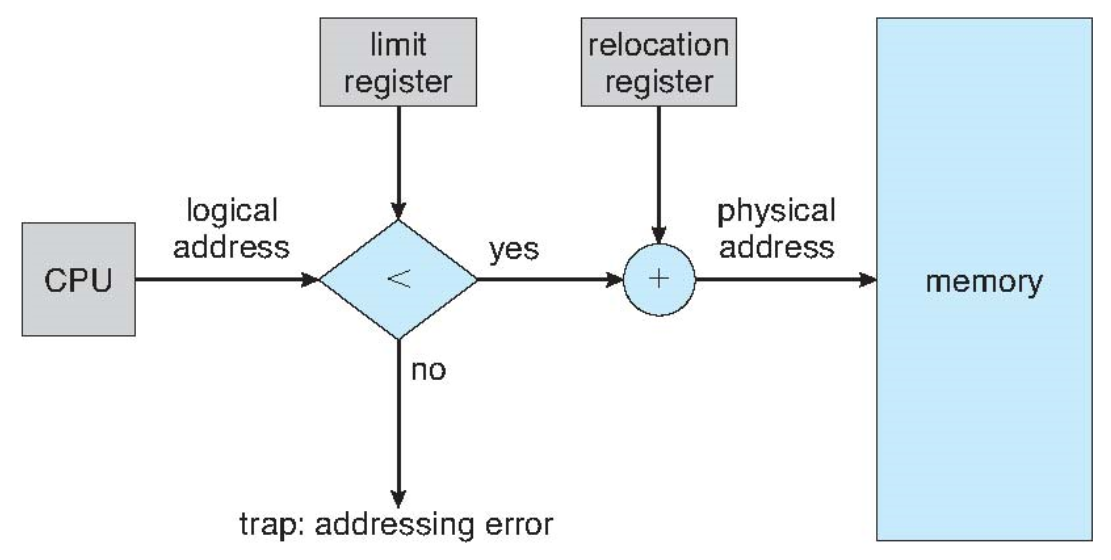
\includegraphics[width=0.65\linewidth]{img/fbs.png}
 \end{figure}


\subsection{Variable Partition}

The OS can decide the Multiple-partition allocation. Degree of multi-programming limited by the number of partitions.

\begin{itemize}
    \item \textbf{Variable-partition} - sizes for efficiency (sized to a given process’ needs).
    \item \textbf{Hole} – block of available memory; holes of various size are scattered throughout memory. Undesired, on paper, you want a continuous block of available memory.
\end{itemize}

\paragraph{}
\newpage
When a process arrives, it is allocated memory from a hole large enough to
accommodate it, when a  process exiting frees its partition, adjacent free partitions combined and all of this is managed by the operating system that maintains information about:

\begin{itemize}
    \item allocated partitions
    \item free partitions (hole)
\end{itemize}

\begin{figure}[htbp]
    \centering
    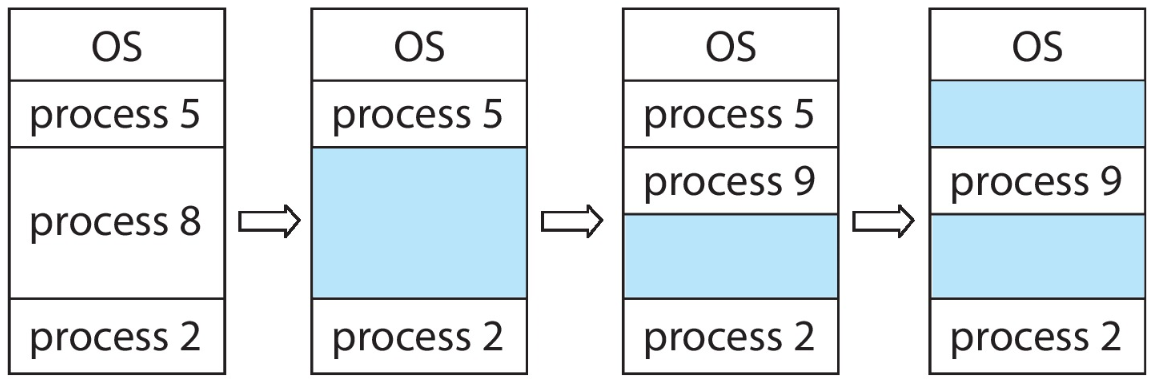
\includegraphics[width=0.5\linewidth]{img/jyrt.png}
\end{figure}


\subsection{Dynamic Storage-Allocation Problem}
How to satisfy a request of size n from a list of free holes?

\begin{itemize}
    \item First-fit: Allocate the first hole that is big enough
    \begin{itemize}
        \item[] May produce many small leftover holes
    \end{itemize}

    \item Best-fit: Allocate the smallest hole that is big enough; must search entire list, unless ordered by size 

    \begin{itemize}
        \item[] Produces the smallest leftover hole, this hole could be not filled anymore.
    \end{itemize}

    \item Worst-fit: Allocate the largest hole; must also search entire list 
    \begin{itemize}
        \item[] Produces the largest leftover hole, it can be filled by other processes.
    \end{itemize}
\end{itemize}

First-fit and best-fit better than worst-fit in terms of speed and storage
utilization.
\newpage
\subsection{Fragmentation}

\paragraph{External Fragmentation } – total memory space exists to satisfy a request, but it is not contiguous. Whether you apply a first-fit or best-fit memory allocation strategy it’ll cause external fragmentation.

\begin{figure}[htbp]
    \centering
    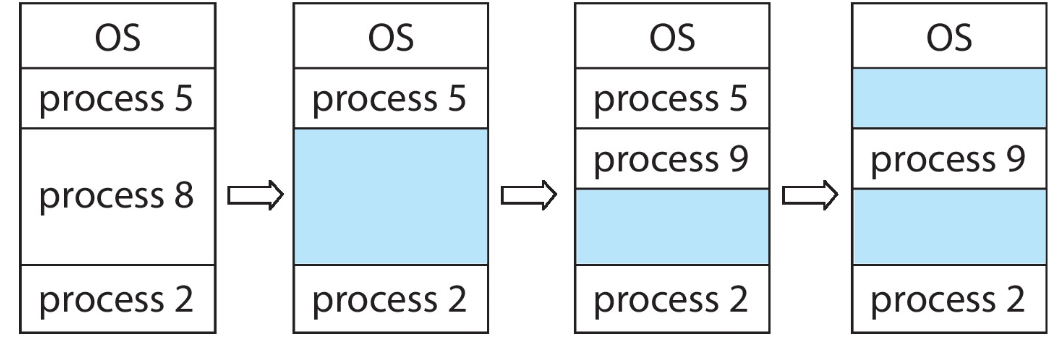
\includegraphics[width=0.5\linewidth]{img/mkjhg.png}
\end{figure}

\paragraph{Internal Fragmentation} – allocated memory may be slightly larger
than requested memory, the minumim  size is defined by the OS and the difference between the C programm and this minimum size is defined Internal Fragmentation.  If we use dynamic partitioning to allot space to the process, this issue can be solved.

\begin{figure}[htbp]
    \centering
    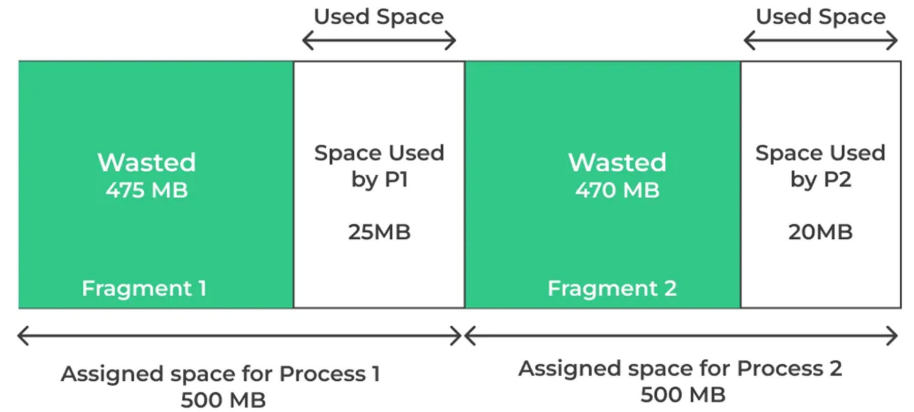
\includegraphics[width=0.65\linewidth]{img/mht.png}
\end{figure}

\subsection{Compaction}
Reduce external fragmentation by \textbf{compaction}, shuffle memory contents to place all free memory together in one large block. Compaction is possible only if relocation is dynamic, and is done at execution time.

\paragraph{}
Although the compaction technique is very useful in making memory utilization efficient and reduces external fragmentation of memory, the problem with it is that a large amount of time is wasted in the process and during that time the CPU sits idle hence reducing the efficiency of the system.
\newpage
\section{Paging}
Suppose that we allow the physical address space of a process can be noncontiguous, the benefit is more. Thus, the process is allocated physical memory whenever the main memory is available. We avoid external fragmentation and varying sized memory chunks.

The paging process consists to divide the physical memory into fixed-sided blocks called \textbf{frame}, the size is a power of 2, between 512 bytes and 16 MiB, also the logical memory is divide in the same size blocks called \textbf{pages}.

\paragraph{NOTE: } is indifferent at this point to talk about if it is a SSD or RAM, is the same, only change the latency and the volatile.

This can allow to keep track all free frames and this can use to run a program of size N pages, need to find N free frames and
load program. To do this we must we set up a page table to translate logical to physical addresses. 
\paragraph{}
We still have Internal fragmentation.

\subsection{Address Translation Scheme}

(Virtual) Address generated by CPU is divided into:

\begin{itemize}
    \item \textbf{Page number (p)} – used as an index into a page table which contains base address of each page in physical memory;
    \item \textbf{Page offset (d)} – combined with base address to define the physical memory address that is sent to the memory unit.
\end{itemize}


\begin{figure}[htbp]
    \centering
    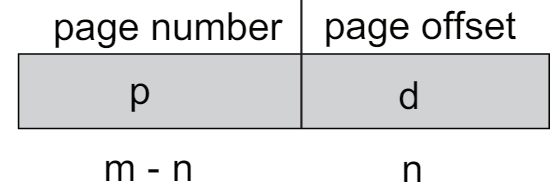
\includegraphics[width=0.4\linewidth]{img/yuj,.png}
\end{figure}

For given logical address space $2^m$ and page size $2^n$.

\newpage
\section{Paging Hardware}

\begin{figure}[htbp]
    \centering
    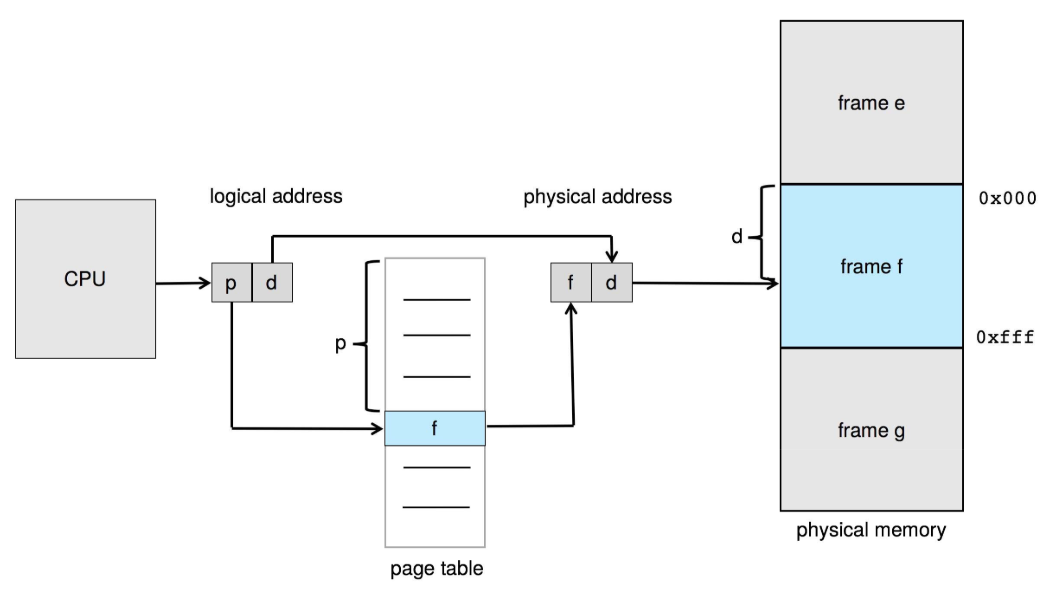
\includegraphics[width=0.6\linewidth]{img/nfg.png}
\end{figure}

\begin{figure}[htbp]
    \centering
    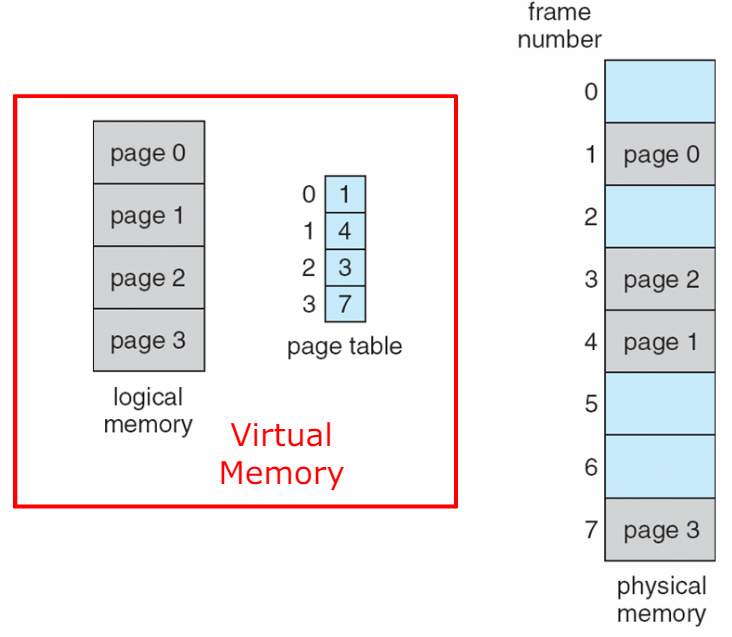
\includegraphics[width=0.5\linewidth]{img/dsf.png}
    \caption{Paging Model of Logical and Physical Memory}
\end{figure}

\newpage
\subsubsection{Paging Example}

Logical address: n = 2 (offset bits), n-m = 3 (page bits). Using a page size of 4 bytes and a physical memory of 32 bit ($2^m$ = 8 pages).

\begin{figure}[htbp]
    \centering
    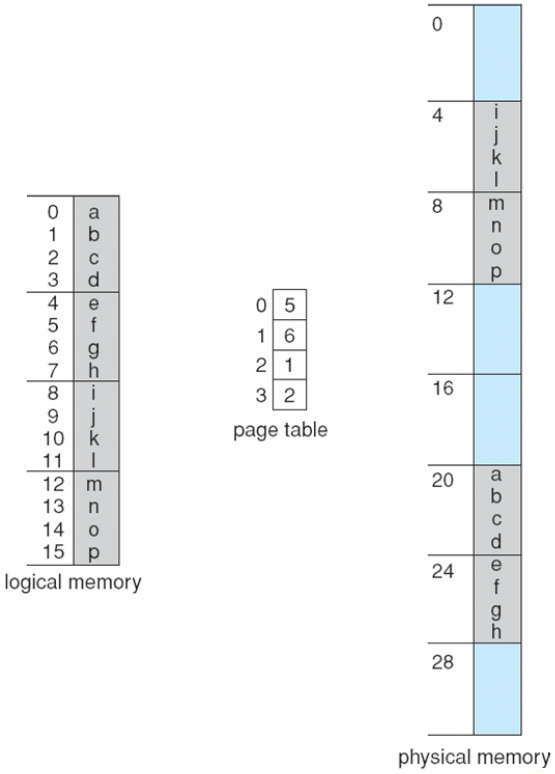
\includegraphics[width=0.5\linewidth]{img/jmy.png}
\end{figure}


\paragraph{Paging - Calculating internal fragmentation}
\paragraph{}
Page size = 2,048 bytes; Process size = 72,766 bytes, we use 35 pages + 1,086 bytes, the internal fragmentation of 2,048 - 1,086 = 962 bytes.

Worst-case scenario = frame size – 1 byte, on average fragmentation = 1 / 2 frame size.

\paragraph{}
Thus, small frame sizes allow for small internal fragmentation...but the page size became bigger because each page table, per process, takes memory to track: Small page size = many many pages = many memory allocated to track the page and unused for the user/OS tasks.

Page sizes growing over time:

\begin{itemize}
    \item Solaris supports two page sizes – 8 KB and 4 MB
    \item Win10 supports two page sizes – 4 KB and 2 MB
    \item Linux supports two page sizes – 4 KB and custom huge page size
\end{itemize}
\newpage
\subsection{How many pages?}
Suppose 4KB (212 bytes) of page size and 32bit hardware CPU. The page table entry is equal to 32 bits. $2^{32}$ pages, each page is 4KiB, the total of memory addressed is 16 TiB ($2^{12} * 2^{10}$, first is the paging addresses and the second is the offset).

\paragraph{}
Another example:
\paragraph{}

\begin{itemize}
\centering
    \item[] m = length address = 8 bits.
    \item[] n = $log_2(page size)$ = $log_2(32 bytes)$ = 5 bits of offset.
    \item[] m - n = 3 = number of page that I can addresses.
\end{itemize}

If you reduce the size of the page you can addresses more pages, and the offset decreases. Normally m = 32 and the page size is 4KiB, like in the previous example.


\begin{figure}[htbp]
    \centering
    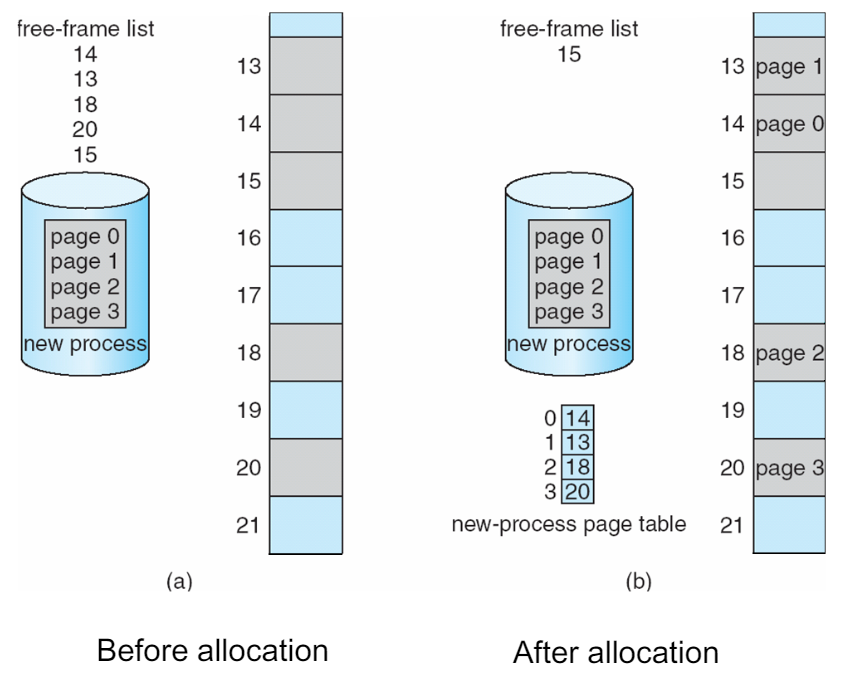
\includegraphics[width=0.7\linewidth]{img/yrtjn.png}
    \caption{Free Frames}
\end{figure}


\subsection{Implementation of Page Table}
Page table, as we said before, is kept in main memory. It is the main “artifact” of the virtual memory management:

\begin{itemize}
    \item[] Page-table base register (PTBR) points to the page table
    \item[] Page-table length register (PTLR) indicates size of the page table
\end{itemize}

In this scheme every data/instruction access requires two memory accesses! One for the page table and one for the data / instruction.

The two-memory access problem can be solved by the use of a special fast-lookup hardware cache called translation look-aside buffers, \textbf{TLBs}.

\paragraph{}
Exploits \textbf{Temporal locality}: the tendency of programs to use data items over and again during
the course of their execution.

\subsection{Hardware solution - Translation Look-Aside Buffer}

TLBs store \textbf{address-space identifiers} (ASIDs) in each TLB entry – uniquely identifies each process to provide addres-space protection for that process, Otherwise need to flush at every context switch.

TLBs typically small, 64 to 1024 entries, but faster, thus, it is a fully-associative cache.

On a TLB miss, value is loaded into the TLB for faster access next time, replacement policies must be considered some entries can be wired down for permanent fast access.

\paragraph{}
It does not speed up everything:

\begin{itemize}
    \item Average case: access in TLB + access in memory for data;
    \item Worst case: no data in TLB, thus access in memory for page table + access in memory for data.
\end{itemize}

\begin{figure}[htbp]
    \centering
    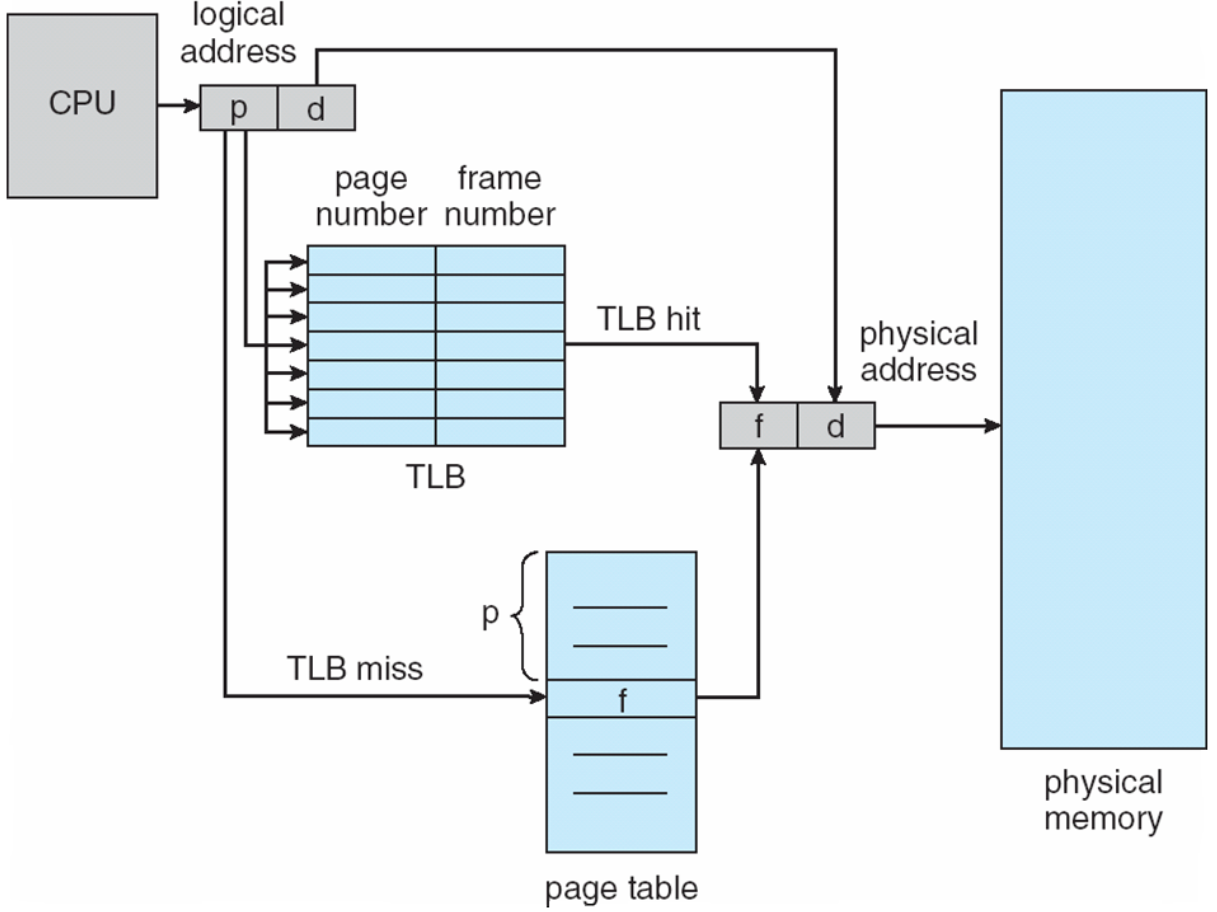
\includegraphics[width=0.6\linewidth]{img/ythmu.png}
\end{figure}

\subsection{Effective Access Time}

\textbf{Hit ratio} – percentage of times that a page number is found in the TLB. An 80\% hit ratio means that we find the desired page number in the
TLB 80\% of the time.

Suppose that you need 10 nanoseconds to access memory. If we find the desired page in TLB then a mapped-memory access take 10 ns, otherwise we need two memory access so it is 20 ns.

\paragraph{}
\textbf{Effective Access Time}, ETA = 0.80 x 10 + 0.20 x 20 = 12 nanoseconds, implying 20\% slowdown in access time.

Consider a more realistic hit ratio of 99\%, EAT = 0.99 x 10 + 0.01 x 20 = 10.1ns, implying only 1\% slowdown in access time.

\newpage
\section{C code and page faults}

Think to have the RAM full, only one page is empty, and in this page we want to do this:

\begin{codeInC}
int main(){
    int[128,128] data;

    ...

    for (j = 0; j <128; j++)
        for (i = 0; i < 128; i++)
            data[i,j] = 0;
 
    //how many page faults? 128 * 128 = 16384

    ...

    for (i = 0; i < 128; i++)
        for (j = 0; j < 128; j++)
            data[i,j] = 0;

    //how many page faults? only 128

}   
\end{codeInC}

\textbf{Page faults} - A page fault occurs when a program attempts to access data or code that is in its address space, but is not currently located in the system RAM.

When we access to something into ram the OS brought a block of data from SSD into ram. In the first case the OS take a block but the C code use only the first column; in the second for the OS take a block of data and use all of the column.


\begin{figure}[htbp]
    \centering
    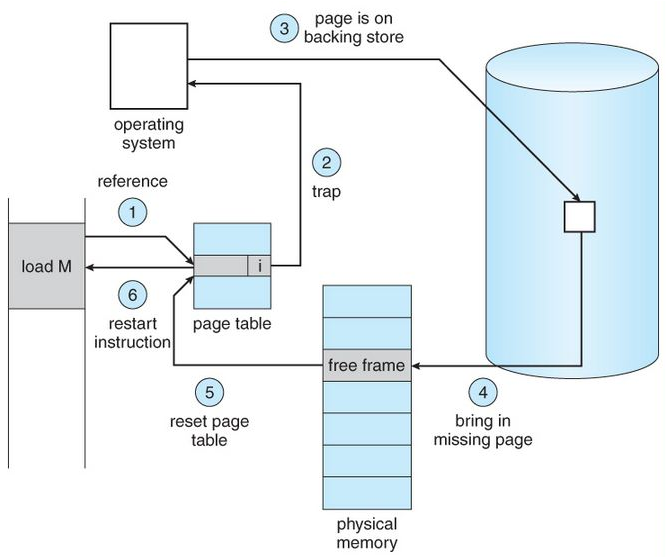
\includegraphics[width=0.65\linewidth]{img/bnetg.png}
    \caption{Page faults}
\end{figure}

\newpage
\section{Page Faults}

\paragraph{What the page faults is?} Data is typically stored in non-volatile big and slow memories and then loaded into RAM, it means that data required for execution (a page) may exist only in the secondary storage due to dynamic loading. Thus it needs to be loaded in the RAM, then cache, then registers, this is a \textbf{page fault}!

\paragraph{}
We can not solve it but we try to mitigate this slow event.

\begin{figure}[htbp]
    \centering
    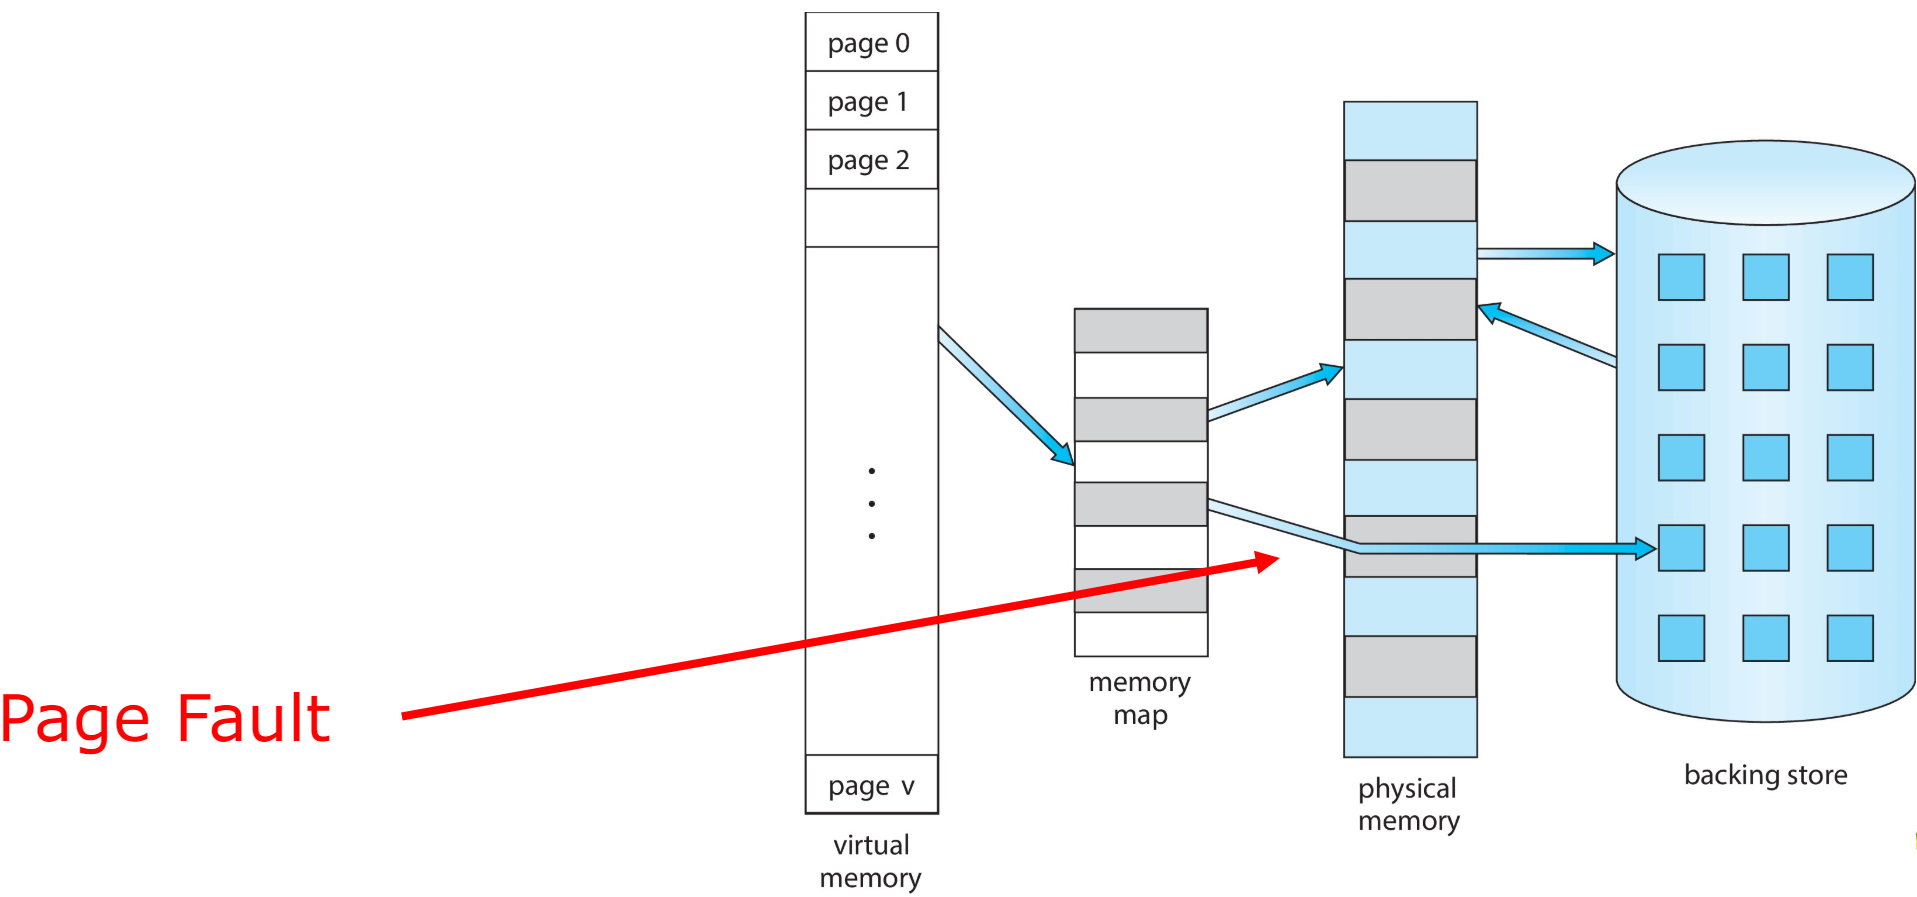
\includegraphics[width=0.75\linewidth]{img/frsb.png}
    \caption{Page fault}
\end{figure}

\subsection{How detecting page faults?}

We can use one bit, \textbf{valid-invalid}, to track is the address is in RAM or in secondary memory.

\begin{itemize}
    \item valid (1): indicate that the associated page is in the process logical address space, and exists in RAM already;
    \item invalid (0): indicates that the page is not in the RAM, it means \textbf{page faults} will happen.
\end{itemize}


\begin{figure}[htbp]
    \centering
    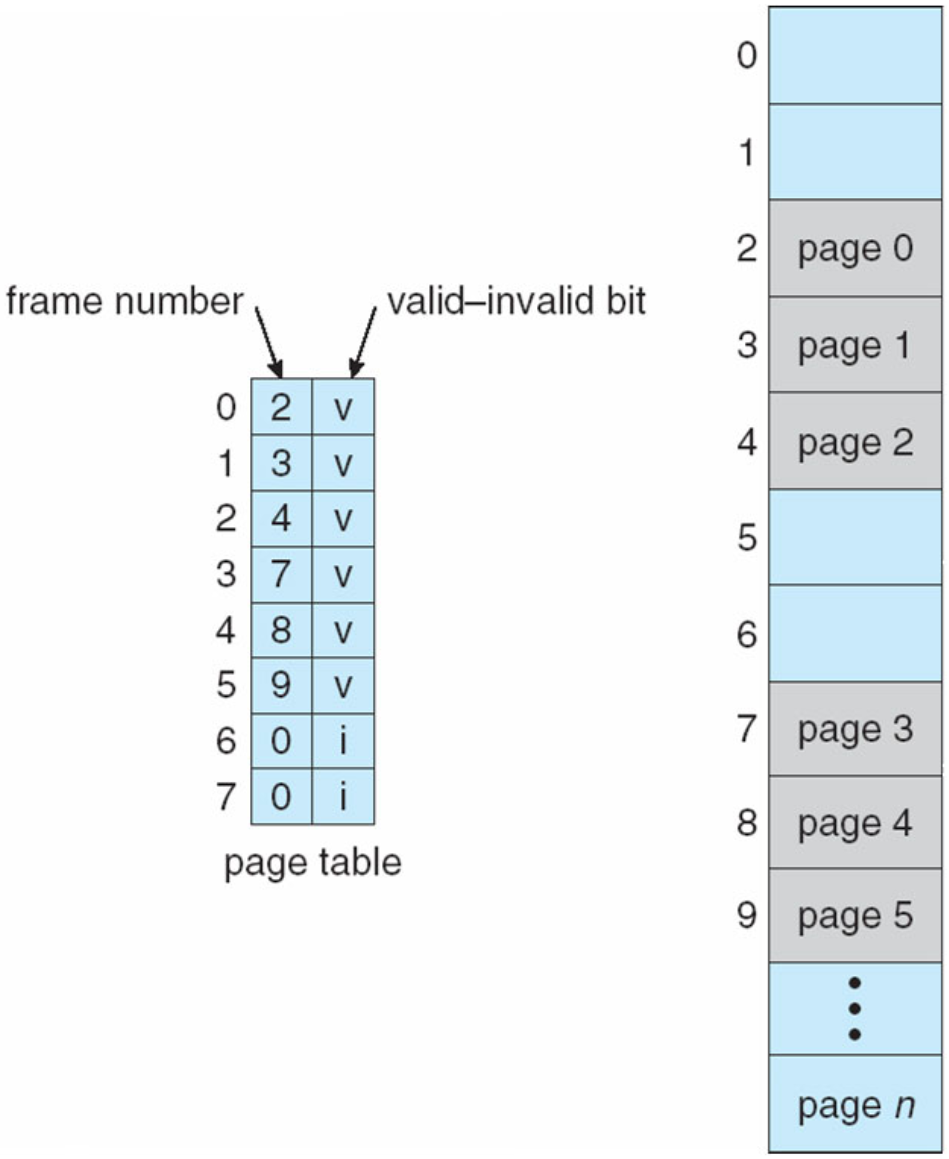
\includegraphics[width=0.5\linewidth]{img/rfynhmg.png}
\end{figure}





\begin{figure}[htbp]
    \centering
    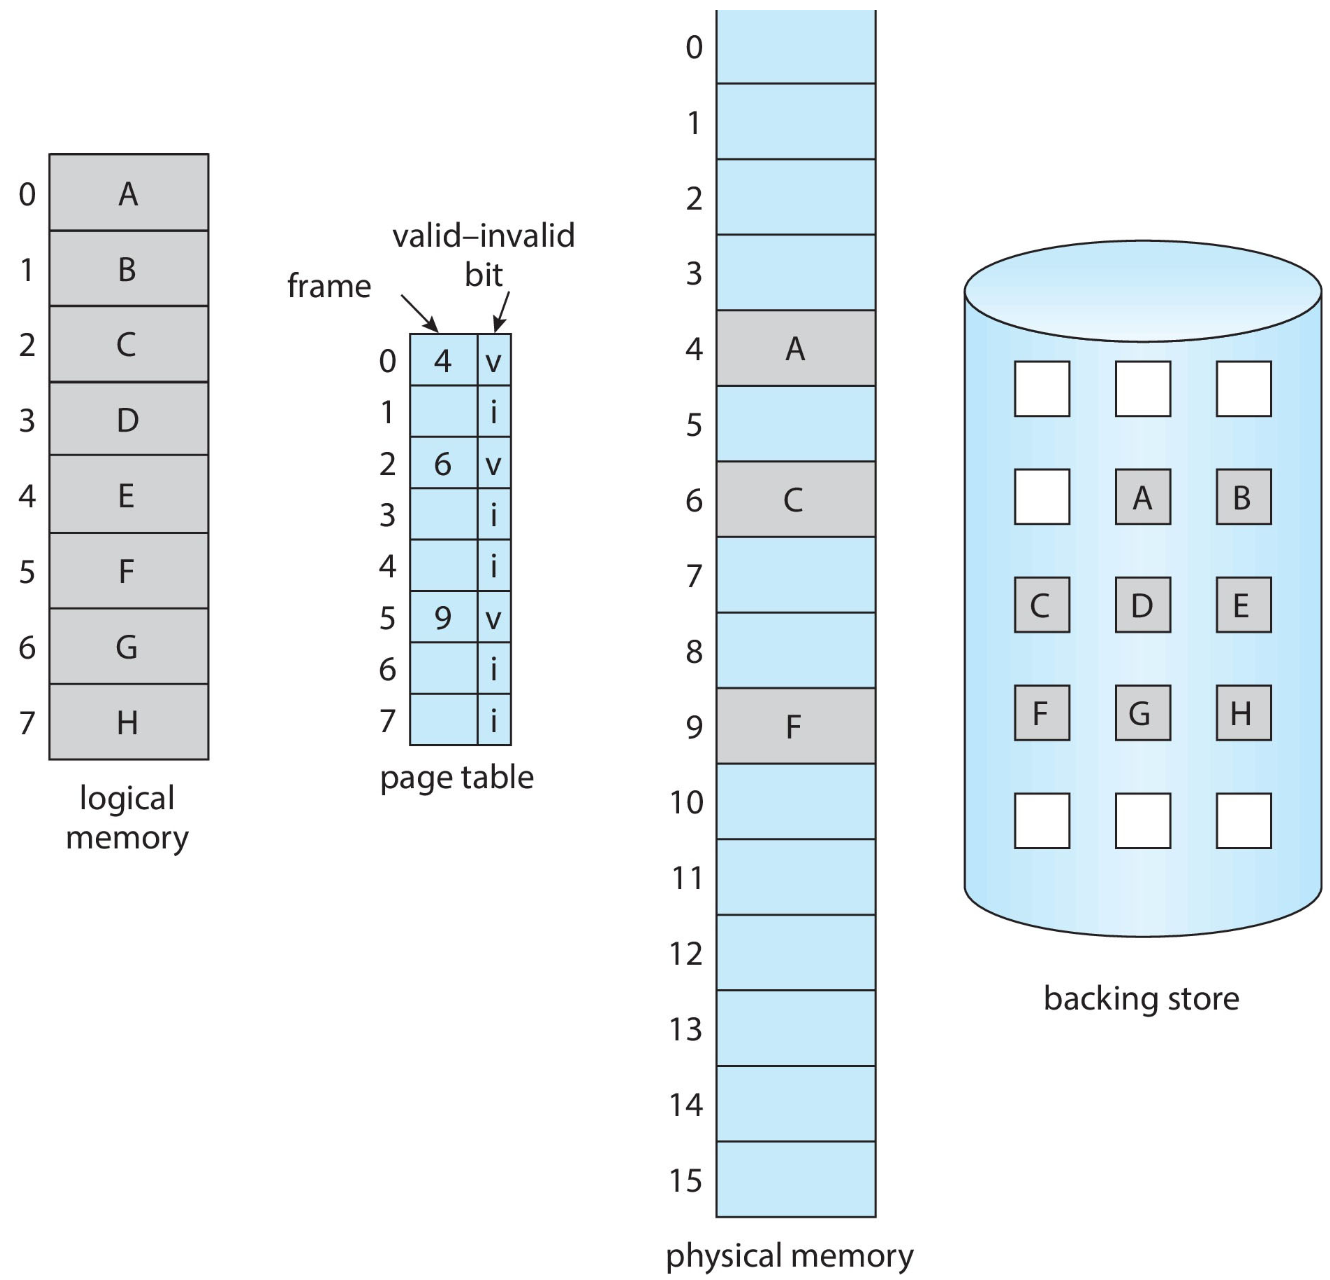
\includegraphics[width=0.5\linewidth]{img/mhg.png}
\end{figure}



\subsection{Steps in handling page faults}

\begin{enumerate}
    \item If there is a reference to a page, first reference to that page will trap to operating system = page faults;
    \item If there is a reference to a page, first reference to that page will trap to operating system;
    \begin{itemize}
        \item[] Invalid reference $\to$ abort
        \item[] Just not in memory, need to be loaded from disk
    \end{itemize}
    \item Find a free frame in memory;
    \item Swap page into frame via scheduled disk operation, the slowest part of the process;
    \item Change tables to indicate page now in memory, Set valid bit = v;
    \item Restart the instruction that caused the page fault;
\end{enumerate}

\begin{figure}[htbp]
    \centering
    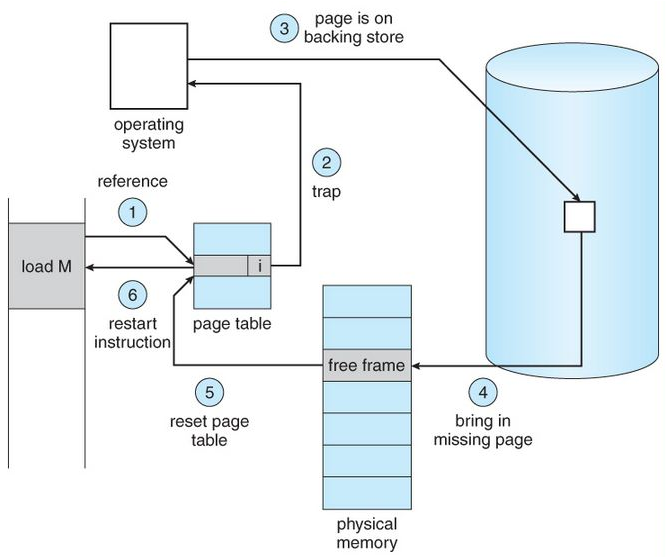
\includegraphics[width=0.6\linewidth]{img/bnetg.png}
    \caption{Page faults}
\end{figure}

\subsection{Cost of a page fault}
Assume of Page Fault Rate 0 < p < 1, if p = 0 no page faults, if p = 1, every reference is a fault.

Effective Access Time:

\begin{itemize}
    \centering 
    \item[] EAT = (1 – p) x memory access + p (page fault overhead)
\end{itemize}

Memory access time = 200 nanoseconds; Average page-fault service time = 8 milliseconds, One access out of 1,000 causes a page fault. It seems a small number but it is not!

\paragraph{}
Assuming of RAM Memory access time = 200 nanoseconds, average page-fault service time = 8 milliseconds:

\begin{itemize}
    \centering 
    \item[] EAT = (1 – p)200 + p (8 milliseconds) = 200 + p7,999,800
\end{itemize}

If one access out of 1,000 causes a page fault, then EAT = 8.2 microseconds. 

This is a slowdown by a factor of 8.2 / 0.2 = 41!! Not very good!

\paragraph{}
This is probably the primary source of slowdowns when computing something.

\newpage
\section{Page replacement strategy}

When a page fault occurs, the operating system must bring the
desired page from secondary storage into main memory. 

Most operating systems maintain a free-frame list -- a pool of free
frames for satisfying such requests.


\begin{figure}[htbp]
    \centering
    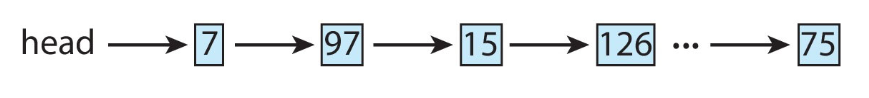
\includegraphics[width=0.5\linewidth]{img/rhsbgfw.png}
\end{figure}

Operating system typically allocate free frames using a technique
known as zero-fill-on-demand -- the content of the frames zeroedout before being allocated. When a system starts up, all available memory is placed on the freeframe list.

\subsection{What Happens if There is no Free Frame?}

Like for scheduling algorithms we can implement the easy solution using random, took a frame in memory put into the HD and the needed page load into RAM, this solution is not the optimal solution!

This technique, beyond the algorithm, is called \textbf{page replacement} - find some page in memory not really in use, push it out and load the needed page.

\paragraph{}
Prevent over-allocation of memory by modifying page-fault service
routine to include page replacement. 

We can do it using \textbf{modify (dirty) bit} to reduce overhead of page transfers – only
modified pages are written to disk.

If the dirty bit is set means that the value in ram change and before load the new page I need to write the value in the HD.

Page replacement completes separation between logical memory and
physical memory – large virtual memory can be provided on a smaller
physical memory.

\paragraph{}

This process means we accesses the HD \textbf{two times}.


\begin{figure}[htbp]
    \centering
    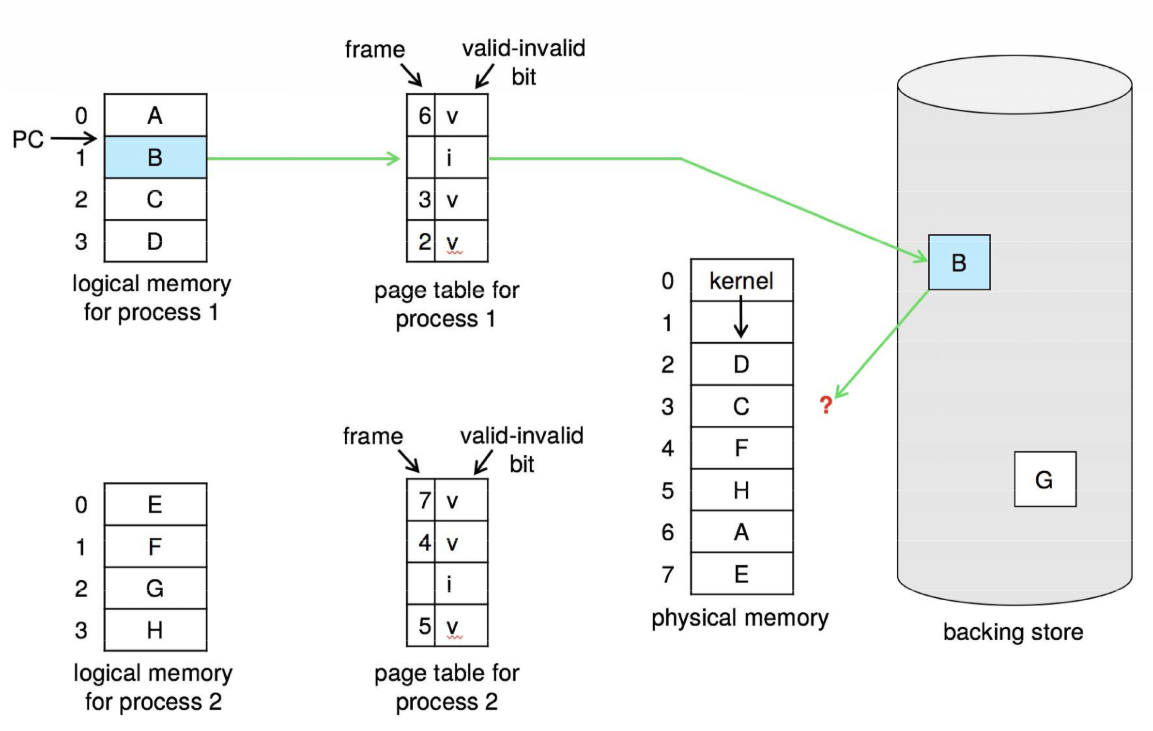
\includegraphics[width=0.75\linewidth]{img/sdfbgv.png}
\end{figure}

\newpage
\subsection{Basic Page Replacement}

\begin{enumerate}
    \item Find the location of the desired page on disk
    \item Find a free frame:
    \begin{itemize}
        \item[]  If there is a free frame, use it
        \item[]  If there is no free frame, use a page replacement algorithm to  select a victim frame
        \item[]  Write victim frame to disk if dirty (= modified while in RAM)
    \end{itemize}
    \item Bring the desired page into the (newly) free frame; update the pageand frame tables
    \item Continue the process by restarting the instruction that caused the trap
\end{enumerate}

\begin{figure}[htbp]
    \centering
    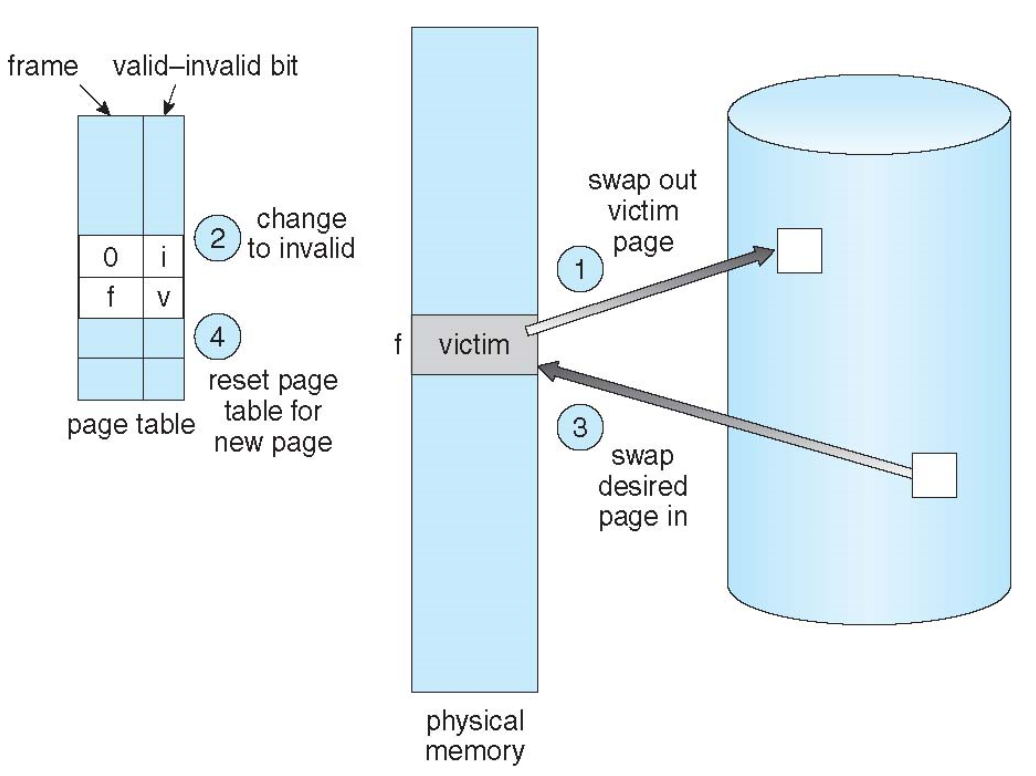
\includegraphics[width=0.65\linewidth]{img/mghj.png}
\end{figure}

\section{Page and Frame Replacement Algorithms}

The Frame-allocation algorithm determines :

\begin{itemize}
    \item[] How many frames to give each process
    \item[] Which frames to replace, ideally I replace only the page that I do not need soon (but It do not predict the future)
\end{itemize}


Page-replacement algorithm: 

\begin{itemize}
    \item[] Want lowest page-fault rate on both first access and re-access
\end{itemize}
\newpage
\begin{figure}[htbp]
    \centering
    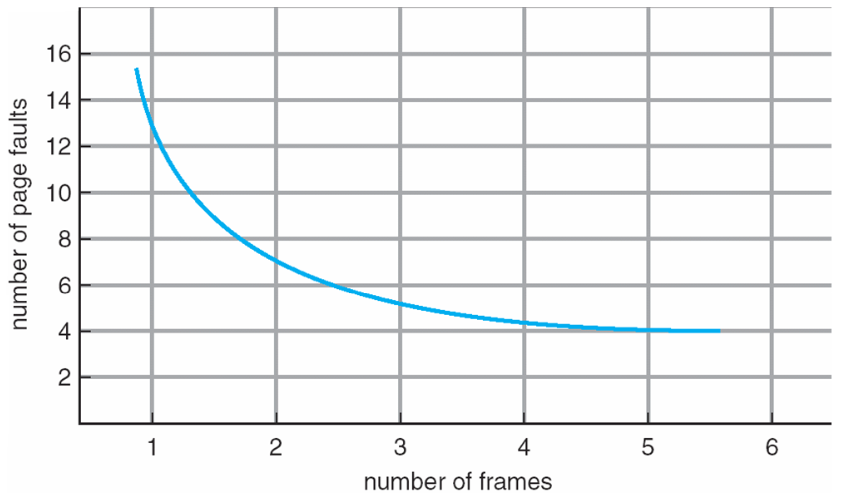
\includegraphics[width=0.65\linewidth]{img/ahet.png}
\end{figure}

In this image we can see that the more frame slots associated to each process, the least the
probability of having page faults.

\subsection{FIFO algorithm}

Reference string: 7,0,1,2,0,3,0,4,2,3,0,3,0,3,2,1,2,0,1,7,0,1; 

3 frames (3 pages can be in memory at a time per process)


\begin{figure}[htbp]
    \centering
    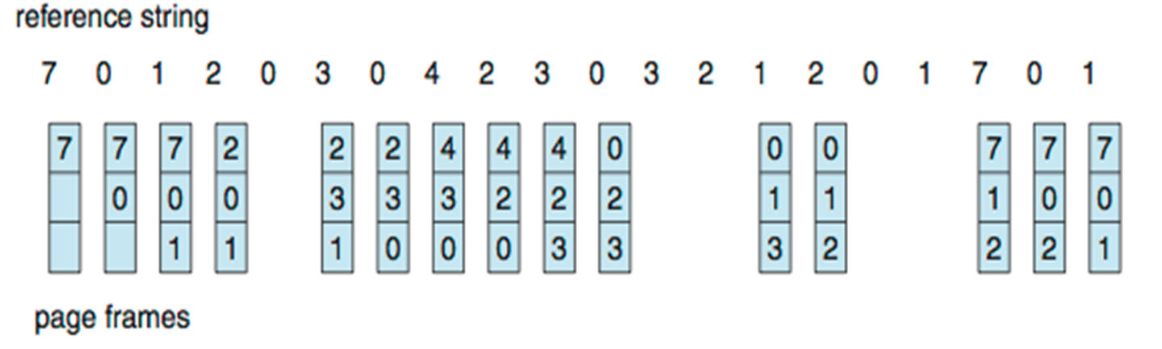
\includegraphics[width=0.75\linewidth]{img/dgnf.png}
\end{figure}

With this methods we have 15 page faults, we can do better?

\subsection{Optimal (?) Algorithm}

Replace page that will not be used for longest period of time, 9 page faults is optimal best for the example. But like sad before we can't read the future, BUT this is the optimal solution so we can measuring how well the algorithm performs. 

\begin{figure}[htbp]
    \centering
    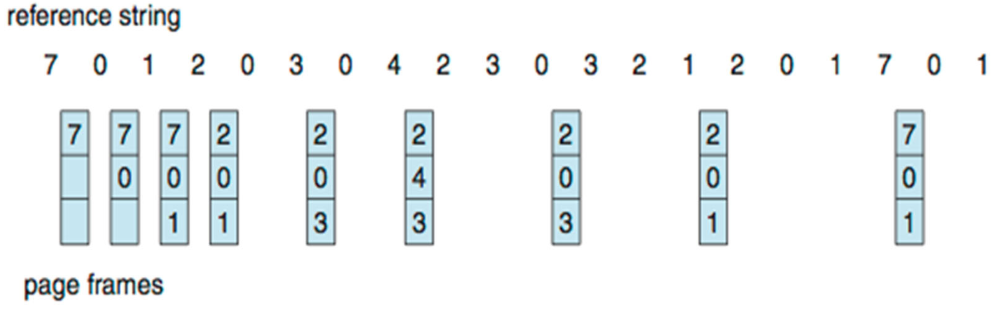
\includegraphics[width=0.77\linewidth]{img/dng.png}
\end{figure}

\newpage
\subsection{Least Recently Used (LRU) Algorithm}

We have seen that the program can not read the future, but we can use the past knowledge rather than future! 

Replace page that has not been used in the most amount of time, exploits principle of temporal locality. Associate time of last use with each page.

\begin{figure}[htbp]
    \centering
    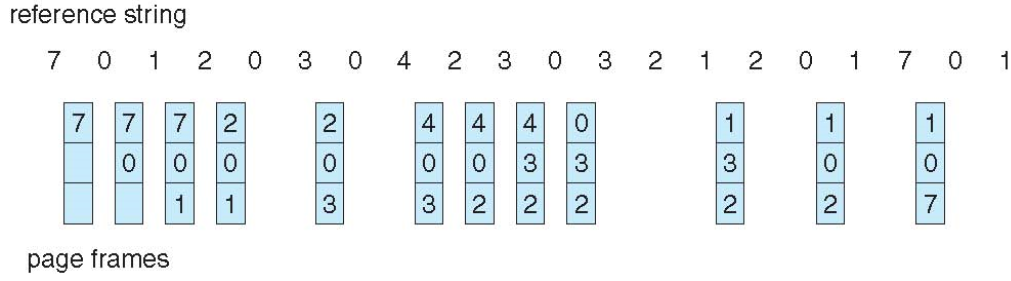
\includegraphics[width=0.8\linewidth]{img/fdb.png}
\end{figure}

12 faults – better than FIFO but worse than OPT; generally good algorithm and frequently used. But how to implement?

\paragraph{Counter implementation: } Every page entry has a counter; every time page is referenced
through this entry, copy the clock into the counter. When a page needs to be changed, look at the counters to find
smallest value, search through table needed.

\paragraph{Stack implementation: } Keep a stack of page numbers in a double link form. Page referenced: move it to the top and requires 6 pointers to be changed.

But each update more expensive and no search for replacement.

\paragraph{}
LRU and OPT are cases of stack algorithms that don’t have
Belady’s Anomaly. Use of a stack to record most recent page references.


\begin{figure}[htbp]
    \centering
    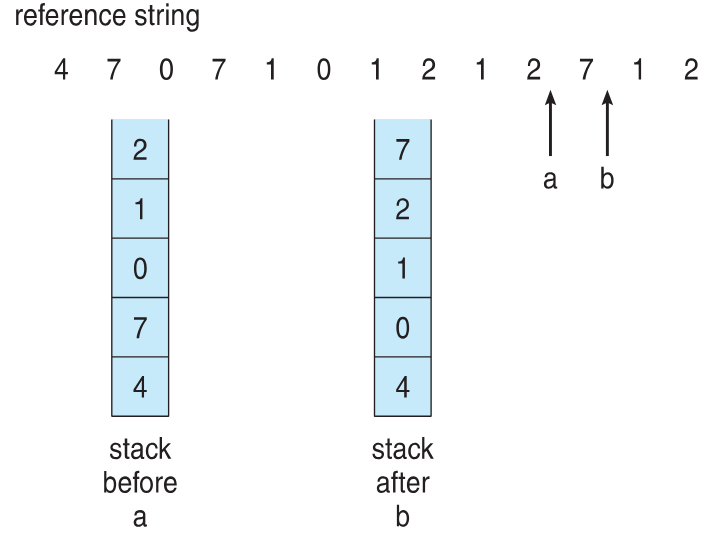
\includegraphics[width=0.6\linewidth]{img/sd.png}
\end{figure}

\newpage
\subsection{LRU Approximation Algorithms}

LRU needs special hardware and still slow and memory (4 bytes each entry). 

We can simplify using only one bit: \textbf{Reference bit}. Initially each page we associate a bit with value 0, than when the page is referenced bit is set to 1. If the OS require memory for process it can replace any page have the bit to value 0 (if one exists).

Worst case scenario, the algo. scroll all the list.

\paragraph{Second-chance algorithm: } Generally FIFO, plus hardware-provided reference bit with \textbf{Clock} replacement. If page to be replaced has:

\begin{itemize}
    \item Reference bit = 0 -> replace it
    \item Reference bit = 1 then:
    \begin{itemize}
    \item[] set reference bit 0, leave page in memory
    \item[] replace next page, subject to same rules
    \end{itemize}
\end{itemize}


\begin{figure}[htbp]
    \centering
    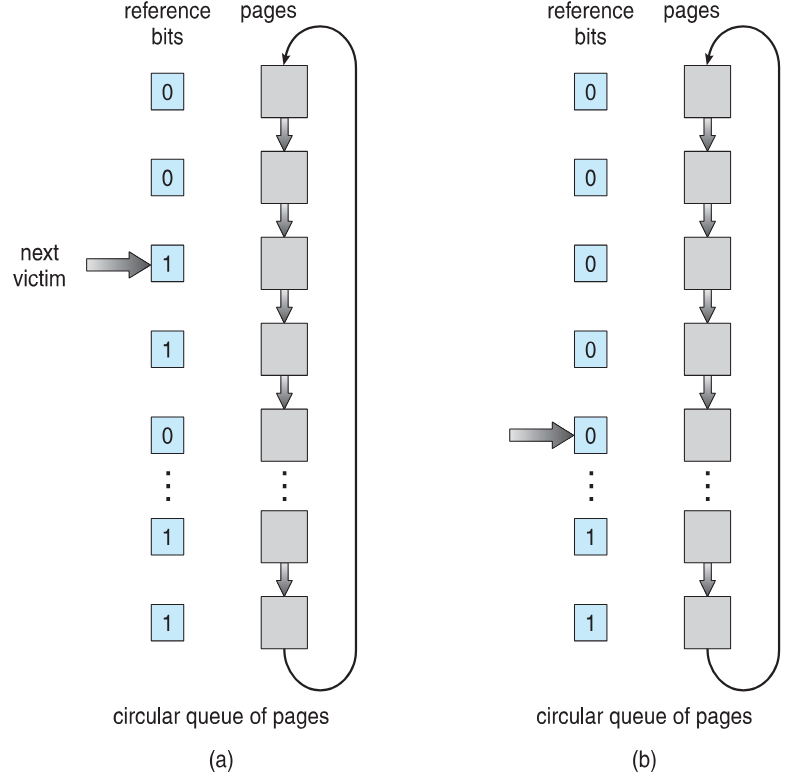
\includegraphics[width=0.65\linewidth]{img/jnyfg.png}
\end{figure}

\subsection{Counting Algorithms}
Keep a counter of the number of references that have been made
to each page, not common.

\subsubsection{Least Frequently Used (LFU) Algorithm:}

\begin{itemize}
    \item Replaces page with smallest count
    \item May have the problem of always replacing the “newly arrived pages” that have the counter set to 1
\end{itemize}


\subsubsection{Most Frequently Used (MFU) Algorithm: }

Based on the argument that the page with the smallest count was probably just brought in and has yet to be used



\section{Allocation of frames to precesses}

Each process needs minimum number of frames, the Maximum of course is total frames in the system. 

Two major allocation schemes: fixed allocation and priority allocation, but also many variations.

\subsection{Fixed Allocation}

For example, if there are 100 frames (after
allocating frames for the OS) and 5 processes, give each process 20
frames. Keep some as free frame buffer pool.

\subsection{Proportional Allocation}

Allocate according to the size of process, dynamic as degree of multiprogramming, process sizes change


In each two allocation there are no way to account for high/low priority tasks.
Whereas ideally you want them to finish early, thus giving them more
memory/CPU

\subsection{Global vs. Local Allocation}

\textbf{Global replacement} – process selects a replacement frame from the set of all frames.

\begin{itemize}
    \item one process can take a frame from another
    \item process execution time can vary greatly
    \item greater throughput so more common
\end{itemize}

\textbf{Local replacement} – each process selects from only its own set of
allocated frames

\begin{itemize}
    \item More consistent per-process performance
    \item possibly underutilized memory
    \item Thus, smaller throughtput
\end{itemize}

\newpage
\subsection{Reclaiming Pages}
A strategy to implement global page-replacement policy is: all memory requests are satisfied from the free-frame list, rather than waiting for the list to drop to zero before we begin
selecting pages for replacement, the Page reclaiming is triggered by the kernel when the list falls below a
certain threshold.

\paragraph{}
The kernel process that manages it is called \textbf{reaper}.

This strategy attempts to ensure there is always sufficient free
memory to satisfy new requests, or the free-frame list is never empty.

\begin{figure}[htbp]
    \centering
    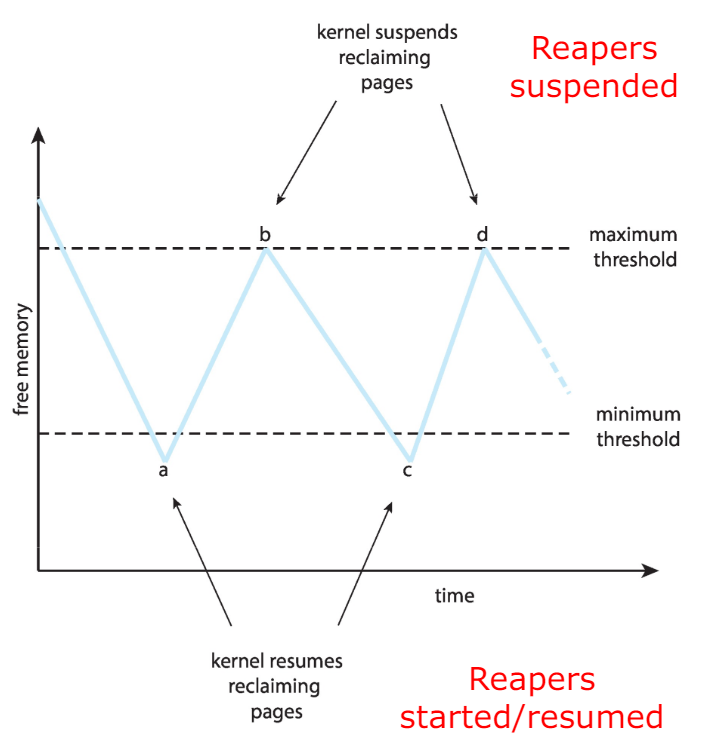
\includegraphics[width=0.6\linewidth]{img/andg.png}
    \caption{Reclaiming Pages Example }
\end{figure}


\newpage
\subsection{Thrashing}

\textbf{Thrashing} - a process is busy swapping pages in and out.
\paragraph{}

If a process does not have “enough” pages, the page-fault rate is very
high: \textbf{Page fault} to get page, \textbf{Replace} existing frame, But quickly need \textbf{replaced frame} back.

All of this cycles leads to:

\begin{itemize}
    \item Low CPU utilization
    \item Operating system thinking that it needs to increase the degree of multiprogramming
    \item Another process added to the system
\end{itemize}

\begin{figure}[htbp]
    \centering
    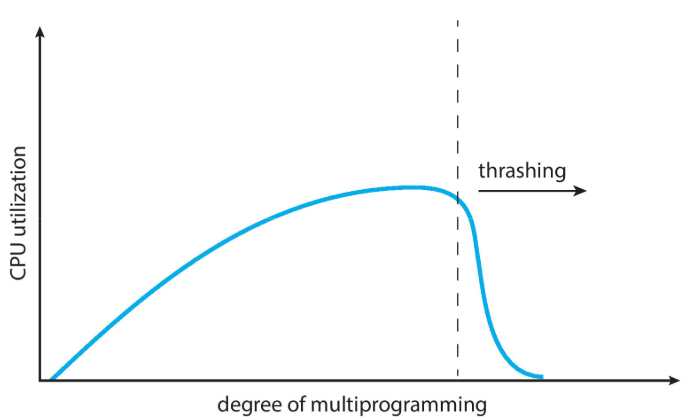
\includegraphics[width=0.5\linewidth]{img/SDBF.png}
\end{figure}

\subsection{Page-Fault Frequency}

Establish “acceptable” page-fault frequency (PFF) rate and use local replacement policy.

\begin{itemize}
    \item[] If actual rate too low, process loses frame
    \item[] If actual rate too high, process gains frame
\end{itemize}

\begin{figure}[htbp]
    \centering
    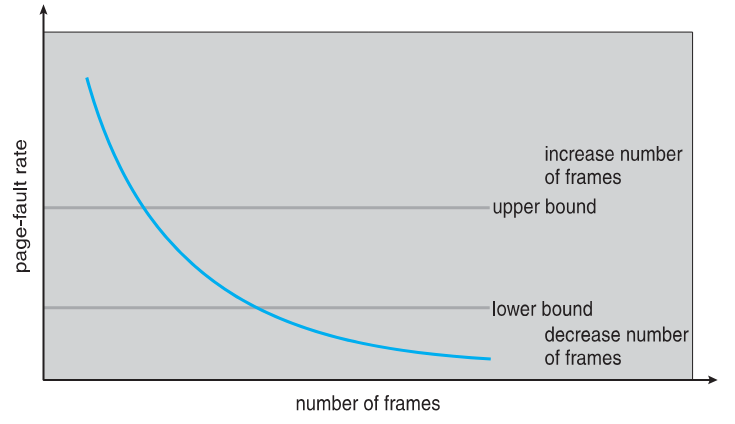
\includegraphics[width=0.5\linewidth]{img/fmh.png}
    \caption{PPF}
\end{figure}
















